\chapter{Weber Electrodynamics}
\section{The Equation of Weber Electrodynamics}
\label{sec:weber_em}
Weber electrodynamics presents an alternative formulation of electromagnetic interactions based on an extension of Coulomb's law (Eq. \ref{eq:weber_em_skalar}).

This equation describes the force between two charges $q_1$ and $q_2$, where $r$ is their separation distance, $\dot{r}$ the relative velocity, $\ddot{r}$ the relative
acceleration, and $c$ the speed of light. The first term corresponds to the classical Coulomb force, while the additional terms account for velocity- and acceleration-dependent
effects.

\subsection{Momentum and Energy}
In Weber electrodynamics, momentum and energy transfer are described directly through the interaction between charges. The total energy of the system consists of the potential
energy of the Coulomb interaction and the kinetic terms of relative motion:

\begin{equation}
    E = \frac{1}{2} m_1 v_1^2 + \frac{1}{2} m_2 v_2^2 + \frac{q_1 q_2}{4 \pi \epsilon_0 r} \left[ 1 - \frac{\dot{r}^2}{2c^2} \right]    
\end{equation}

This formulation shows how Weber's theory ensures energy conservation even in dynamic processes.

\subsection{Speed of Light and Space Model}
A central aspect of Weber electrodynamics is its treatment of the speed of light $c$. Unlike \gls{srt}, which postulates $c$ as an absolute constant,
$c$ appears in Weber's theory as a parameter determining the propagation speed of interactions. This allows for a space model where the speed of light
is interpreted not as a universal limit but as a property of the interaction itself.

\subsection{Advantages of Weber Electrodynamics}
Weber electrodynamics offers several conceptual advantages:
\begin{enumerate}
    \item \textbf{Elimination of Fields:}\\Since interactions are described directly between charges, the need for a mediating field entity is eliminated.
    \item \textbf{Consistent Action at a Distance:}\\The theory unites instantaneous and retarded effects in a single equation, resolving the apparent contradictions of classical action at a distance.
    \item \textbf{Energy Conservation:}\\The Weber force automatically ensures conservation of energy and momentum without additional assumptions.
    \item \textbf{Alternative Representation:}\\The theory provides a way to describe electromagnetic phenomena without the postulates of special relativity.
\end{enumerate}

Weber electrodynamics represents an elegant and consistent alternative to conventional field theory. By combining instantaneous and retarded effects, it enables
a deeper understanding of electromagnetic interactions and opens new perspectives on fundamental physics questions, such as the nature of the speed of light and the structure
of space.

\section{Comparative Example Calculations}
\subsection{Force Between Uniformly Moving Charges}

\textbf{Scenario:} Two point charges $q_1 = q_2 = e$ (elementary charge) move parallel at $v = 0.1c$ with separation $d = 1\,\text{\AA}$.

\begin{table}[ht]
\centering
\caption{Force Calculation Comparison}
\begin{tabular}{lcc}
\toprule
 & \textbf{Maxwell} & \textbf{Weber} \\
\midrule
Coulomb Term & $\displaystyle\frac{e^2}{4\pi\epsilon_0 d^2}$ & $\displaystyle\frac{e^2}{4\pi\epsilon_0 d^2}\left(1-\frac{v^2}{c^2}\right)$ \\
Magnetic Term & $\displaystyle\frac{\mu_0 e^2 v^2}{4\pi d^2}$ & -- \\
\hline
Force Asymmetry & $2F_B = 5.12\times10^{-11}\,\text{N}$ & $0$ \\
\bottomrule
\end{tabular}
\end{table}

\begin{equation}
    F_{\text{Weber}} = \frac{e^2}{4\pi\epsilon_0 d^2}\left[1 - \frac{v^2}{c^2}\right] \approx 2.29\times10^{-8}\,\text{N}
\end{equation}

\subsection{Radiation Damping of Harmonic Oscillation}

For an electron with $x(t) = x_0\cos(\omega t)$:

\begin{align}
    \label{eq:weber-em-damp}
    \textbf{Maxwell:}\quad & P = \frac{e^2\omega^4 x_0^2}{6\pi\epsilon_0 c^3}\cos^2(\omega t) \\
    \textbf{Weber:}\quad & F_{\text{damp}} = -\frac{e^2\omega^2\dot{x}}{4\pi\epsilon_0 c^3}
\end{align}

\begin{figure}[ht]
\centering
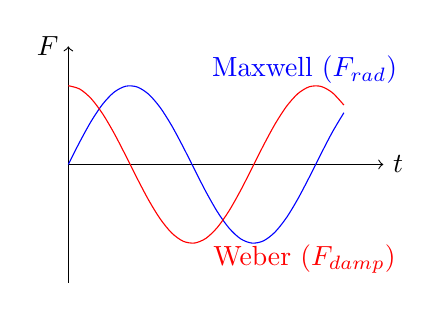
\begin{tikzpicture}
\draw[->] (0,0) -- (4,0) node[right]{$t$};
\draw[->] (0,-1.5) -- (0,1.5) node[left]{$F$};
\draw[domain=0:3.5,smooth,variable=\x,blue] plot ({\x},{sin(2*\x r)});
\draw[domain=0:3.5,smooth,variable=\x,red] plot ({\x},{cos(2*\x r)});
\node[blue] at (3,1.2) {Maxwell ($F_{\text{rad}}$)};
\node[red] at (3,-1.2) {Weber ($F_{\text{damp}}$)};
\end{tikzpicture}
\caption{Time dependence of reaction forces}
\end{figure}

\subsection{Interpretation of Results}

\begin{itemize}
\item \textbf{Action=Reaction:}\\While Maxwell's theory shows a $2F_B$ asymmetry in the magnetic force component, Weber electrodynamics maintains symmetry.

\item \textbf{Radiation Damping:}\\Weber's theory provides a local description of damping without the causal paradoxes of the Abraham-Lorentz force:

\begin{equation}
\tau_{\text{Weber}} = \frac{e^2}{4\pi\epsilon_0 m c^3} \approx 6.3\times10^{-24}\,\text{s}
\end{equation}

\item \textbf{Energy Conservation:}\\Both theories conserve total energy, but Weber electrodynamics requires no separate field concept.
\end{itemize}

\section{Vector Form of the Weber Force}
\subsection{Derivation from the Scalar Form}

The scalar Weber force (Eq. \ref{eq:weber_em_skalar}) can be generalized by expressing $\dot{r}$ and $\ddot{r}$ in terms of vector quantities.
For the relative vector $\vec{r} = \vec{r}_1 - \vec{r}_2$:

\subsubsection{Conversion of Time Derivatives}
\begin{enumerate}
\item \textbf{First Derivative:}
\begin{equation}
\dot{r} = \frac{d}{dt}\|\vec{r}\| = \frac{\vec{r} \cdot \dot{\vec{r}}}{r} = \hat{\vec{r}} \cdot \vec{v}
\end{equation}
where $\vec{v} = \dot{\vec{r}}$ is the relative velocity and $\hat{\vec{r}} = \vec{r}/r$ the unit vector.

\item \textbf{Second Derivative:}
\begin{align}
\ddot{r} &= \frac{d}{dt}\left(\frac{\vec{r} \cdot \vec{v}}{r}\right) \nonumber \\
&= \frac{\|\vec{v}\|^2 + \vec{r} \cdot \vec{a}}{r} - \frac{(\vec{r} \cdot \vec{v})^2}{r^3} \nonumber \\
&= \frac{v^2 - (\hat{\vec{r}} \cdot \vec{v})^2}{r} + \hat{\vec{r}} \cdot \vec{a}
\end{align}
with $\vec{a} = \dot{\vec{v}}$ the relative acceleration.
\end{enumerate}

\subsection{Complete Vector Form}
Substituting into (Eq. \ref{eq:weber_em_skalar}) yields the \textbf{\enquote{vector form}}:

\begin{equation}
\vec{F}_{12} = \frac{q_1 q_2}{4\pi\epsilon_0 r^2} \left\{
\left[1 - \frac{v^2}{c^2} + \frac{2r(\hat{\vec{r}} \cdot \vec{a})}{c^2}\right]\hat{\vec{r}} + \frac{2(\hat{\vec{r}} \cdot \vec{v})}{c^2}\vec{v}
\right\}
\label{eq:weber_vector}
\end{equation}

\subsection{Physical Interpretation}
The vector form explicitly shows:
\begin{itemize}
\item \textbf{Radial Component:}\\Contains Coulomb term, relativistic correction and acceleration dependence
\item \textbf{Tangential Component:}\\$\propto (\hat{\vec{r}}\cdot\vec{v})\vec{v}$ describes velocity-dependent effects analogous to magnetic fields
\end{itemize}

\subsection{Example Application: Circular Motion}
For a charge $q_2$ with $\vec{v} \perp \vec{r}$ (e.g., circular orbit):

\begin{equation}
\vec{F}_{12} = \frac{q_1 q_2}{4\pi\epsilon_0 r^2} \left[
\left(1 - \frac{v^2}{c^2}\right)\hat{\vec{r}} + \frac{2v^2}{c^2}\hat{\vec{r}}
\right] = \frac{q_1 q_2}{4\pi\epsilon_0 r^2} \left(1 + \frac{v^2}{c^2}\right)\hat{\vec{r}}
\end{equation}

This demonstrates:
\begin{itemize}
\item Additional centripetal force $\propto v^2/c^2$
\item Exact fulfillment of Action=Reaction despite motion
\end{itemize}

\subsection{Graphical Representation of Force Components}

\begin{figure}[ht]
\centering
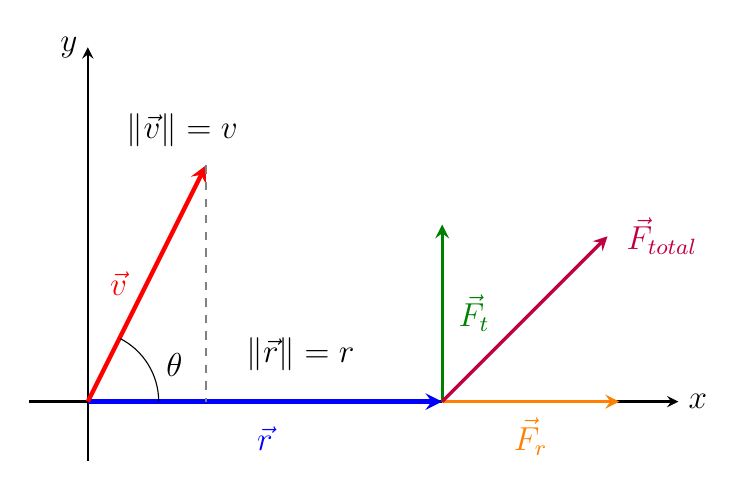
\begin{tikzpicture}[>=stealth,scale=1.5,font=\large]
% Coordinate system
\draw[->,thick] (-0.5,0) -- (5,0) node[right]{$x$};
\draw[->,thick] (0,-0.5) -- (0,3) node[left]{$y$};

% Vectors
\draw[->,ultra thick,blue] (0,0) -- (3,0) node[midway,below=5pt]{$\vec{r}$};
\draw[->,ultra thick,red] (0,0) -- (1,2) node[midway,left=3pt]{$\vec{v}$};
\draw[dashed,gray] (1,2) -- (1,0);

% Force components
\draw[->,very thick,green!50!black] (3,0) -- (3,1.5) node[midway,right=2pt]{$\vec{F}_t$};
\draw[->,very thick,orange] (3,0) -- (4.5,0) node[midway,below=2pt]{$\vec{F}_r$};
\draw[->,very thick,purple] (3,0) -- (4.4,1.4) node[right=3pt]{$\vec{F}_{\text{total}}$};

% Angle
\draw (0.6,0) arc (0:63:0.6) node[midway,right=3pt]{$\theta$};
\node at (1.8,0.4) {$\|\vec{r}\| = r$};
\node at (0.8,2.3) {$\|\vec{v}\| = v$};
\end{tikzpicture}
\caption{Visualization of vector Weber force components. \\
$\vec{F}_r$: Radial component (orange), $\vec{F}_t$: Tangential component (green), \\
$\vec{F}_{\text{total}}$: Total force (purple). The diagram shows the case $\theta = 63^\circ$.}
\label{fig:weber_force}
\end{figure}

\subsection{Vector Component Decomposition}
Based on Fig. \ref{fig:weber_force}, the components are:

\begin{align}
\vec{F}_r &= \frac{q_1 q_2}{4\pi\epsilon_0 r^2}\left[1 - \frac{v^2}{c^2} + \frac{2r a_r}{c^2}\right]\hat{\vec{r}} \\
\vec{F}_t &= \frac{q_1 q_2}{4\pi\epsilon_0 r^2}\left[\frac{2v_r v_t}{c^2}\right]\hat{\vec{t}}
\end{align}

where:
\begin{itemize}
\item $v_r = v\cos\theta$ (radial velocity)
\item $v_t = v\sin\theta$ (tangential velocity)
\item $a_r = \dot{v}_r - v_t^2/r$ (radial acceleration)
\end{itemize}

\subsection{Practical Application Cases}

\textbf{Case 1: Purely Radial Motion ($\theta = 0^\circ$)}
\begin{equation}
\vec{F} = \frac{q_1 q_2}{4\pi\epsilon_0 r^2}\left[1 - \frac{v^2}{c^2} + \frac{2r a}{c^2}\right]\hat{\vec{r}}
\end{equation}

\textbf{Case 2: Circular Motion ($\theta = 90^\circ$)}
\begin{equation}
\vec{F} = \frac{q_1 q_2}{4\pi\epsilon_0 r^2}\left[\left(1 + \frac{v^2}{c^2}\right)\hat{\vec{r}} + \frac{2v^2}{c^2}\hat{\vec{t}}\right]
\end{equation}

\subsection{Advantages Over Maxwell Theory}

\begin{itemize}
    \item \textbf{Nanoplasmonics}
    \begin{itemize}
        \item Exact description of electron-electron interactions in metal clusters ($<10$\,nm)
        \item Avoids infinite self-energy of point charges
        \item More precise modeling of plasmon resonances
    \end{itemize}
    
    \item \textbf{Quantized Vacuum Fields}
    \begin{itemize}
        \item Direct particle interaction without zero-point fluctuations
        \item Natural regularization of vacuum energy density
        \item Alternative to perturbative \gls{qed} calculations
    \end{itemize}
    
    \item \textbf{Dense Plasma Physics}
    \begin{itemize}
        \item More efficient simulation of collective effects
        \item Exact momentum conservation without macro-particle approximation
        \item Better handling of short-range correlations
    \end{itemize}
    
    \item \textbf{Alternative Gravity Theories}
    \begin{itemize}
        \item Consistent coupling to scalar-tensor gravity models
        \item Natural embedding in Machian principles \cite{Assis1999}
        \item Avoidance of singularities in compact objects
    \end{itemize}
\end{itemize}

\subsection{Concrete Examples}

\subsubsection{1. Non-neutral Plasmas in Traps}
For electrons in Penning traps, Weber EM shows:
\begin{equation}
\omega_{\text{Weber}} = \omega_p\sqrt{1 - \frac{3}{4}\frac{v_0^2}{c^2}}
\end{equation}
whereas Maxwell theory predicts $\omega_p = \sqrt{ne^2/\epsilon_0 m}$.

\subsubsection{2. Molecular Dynamics in Strong Fields}
For laser-matter interaction ($>10^{18}\,\text{W/cm}^2$):
\begin{itemize}
\item Weber EM correctly reproduces retarded pair potential form
\item Avoids artifacts of PIC simulations ("self-forces")
\end{itemize}

\subsection{Limitations of Applicability}
\begin{itemize}
\item \textbf{High Energies} ($>100$\,GeV): \gls{qed} effects dominate
\item \textbf{Extended Radiation}: Weber fails for $\lambda \gg \text{particle separation}$
\end{itemize}

\section{Weber Electrodynamics and the EPR Paradox: Two Complementary Approaches}
The apparent confrontation between Weber electrodynamics and \gls{epr} stems from a fundamental tension in modern physics: the struggle for a consistent
understanding of causality and non-locality in classical and quantum systems. This discussion gains particular relevance as both approaches - despite their
different historical contexts - offer alternative perspectives on the problem of action at a distance.

The debate between Weber electrodynamics and \gls{epr} rests on different theoretical paradigms. Weber's theory as a classical action-at-a-distance theory describes
electromagnetic interactions through direct forces between charges, deliberately avoiding field concepts. Wilhelm Weber himself aimed to unify this with Newtonian
principles, particularly strict action-reaction symmetry. As a pre-quantum theory, it makes no claim to explain quantum phenomena.

In contrast, the \gls{epr} paradox emerged in 1935 as a quantum thought experiment to investigate non-local correlations. Subsequent Bell inequalities (Section \ref{sec:bell}) and
their experimental confirmation showed that this quantum entanglement is incompatible with classical locality concepts. Both concepts have their legitimate place in
physics: Quantum mechanics dominates microscopic description, while Weber electrodynamics remains relevant as a historically interesting alternative for classical problems.

\subsection{Non-Locality: Two Physical Manifestations}
The comparative study of both theories gains importance as they exemplify how differently non-locality can be conceptualized in physical models. Both theories exhibit
characteristic non-localities that fundamentally differ. Weber electrodynamics describes classical action at a distance with retarded force propagation (typically at light speed),
where the interaction depends on relative velocity and acceleration of charges. This remains compatible with classical causality and energy conservation.

Quantum mechanics, however, shows instantaneous correlations of entangled states that cannot be explained by any local hidden variables. The crucial difference
lies in the physical mechanism: While Weber's theory postulates deterministic, calculable distant forces, quantum non-locality involves
probabilistic correlations without classical causal structure.

\subsection{Instantaneity and the Concept of Causality}
The current debate about these concepts reflects the fundamental dilemma of modern physics: the contradiction between relativistic locality and quantum
non-locality. Weber electrodynamics demands a reevaluation of causality, as it contains instantaneous components that nevertheless transmit no signals. These terms
rather correspond to structural boundary conditions - mathematical gradients of the potential in configuration space that ensure global consistency. They act as topological
necessities for energetic minimization processes, similar to global conservation laws.

Experimentally, these instantaneous effects cannot be manipulated, just as quantum entanglement allows no superluminal signaling. This perspective shows how seemingly
contradictory principles - local causality and global instantaneity - can be unified in a consistent framework, comparable to Bohm's concept of
\enquote{implicate order} or Penrose's idea of a pre-geometric spacetime.

The ongoing discussion proves that understanding non-locality and causality remains among the central unsolved problems of theoretical physics.
Both approaches - though historically and conceptually distinct - contribute valuable insights to this fundamental question by revealing alternative thought models beyond
the conventional field paradigm.

\section{Space Models}
Modern physics operates with highly precise mathematical descriptions of nature, yet lacks a consistent physical model of space itself. Maxwell's theory of
electromagnetic waves dispenses with the ether but leaves unanswered the question of the actual carrier medium. \gls{art} replaces classical space with a dynamic
spacetime continuum, yet this concept remains an abstract mathematical construction without mechanistic foundation. The singularities in black holes and the
need for dark matter as correction factor indicate profound problems with this approach.

Action-at-a-distance theories like Weber electrodynamics offer a radically different approach by entirely dispensing with a space model and describing interactions directly between particles.
This raises the fundamental question of whether space might not be a primary concept of physics but rather itself an emergent phenomenon. A
promising alternative proposal would be a discrete space model based on a dodecahedral structure. Such a model could not only explain the puzzling \enquote{axis of evil} in the
cosmic microwave background but also make constants like the speed of light understandable as byproducts of the underlying lattice dynamics.

The key concept of this new perspective is emergence - the notion that known physical laws are not fundamental but arise from a deeper underlying
structure. \gls{srt} with its constant speed of light would then reveal itself as a macroscopic effect of discrete space structure, similar
to how thermodynamics emerges from statistical mechanics. The curvature of spacetime in General Relativity would appear no longer as a primary property but
as a coarse-grained description of distortions in the fundamental dodecahedral network.

Particularly noteworthy is the possibility of describing particle properties through topological invariants like Jones polynomials. These mathematical
structures from knot theory could bridge discrete space geometry and quantum phenomena without resorting to conventional quantum field concepts. In this
way, even the dark matter problem might be circumvented, with observed galaxy rotations following directly from lattice dynamics.

Physics stands at a crossroads between two fundamentally different approaches. On one side are theories like General and Special Relativity, which work with a
mathematically defined space model - an abstract spacetime that curves and stretches. While these theories can accurately predict phenomena like gravitational waves,
they remain ultimately descriptive: They describe how nature behaves without explaining why it behaves that way. The spacetime of \gls{art} is a pure computational construct that
works but whose physical manifestation remains obscure. It is as if one could perfectly predict the movement of shadows on a wall without ever understanding the objects
that cast them.

In contrast, action-at-a-distance theories like Weber electrodynamics offer a radically different approach. By entirely dispensing with a space model and describing interactions directly between particles,
they avoid the ontological pitfalls of relativity theories. This approach is in some ways more modest - it makes no claim to force nature into a
prefabricated mathematical straitjacket. Instead, it follows the principle that our theories should not prescribe nature's laws but that nature itself should determine
which regularities are possible.

This difference is fundamental. \gls{art}/\gls{srt} start from mathematical ideality and attempt to press nature into this ideal. The action-at-a-distance approach, however,
begins with observable phenomena and develops its description from them - a method much closer to the true spirit of scientific empiricism. It is the difference
between an architect who imposes his visions on the landscape and a gardener who works with the given conditions of the soil.

The fact that action-at-a-distance theories can make precise predictions without any space model should give us pause. It shows that our preference for visualizable
models may have more to do with our cognitive limitations than with nature itself. Perhaps space is indeed nothing more than a useful concept emerging from
deeper principles - just as temperature arises from particle motion without being a fundamental concept itself.

Relativity theories have undoubtedly achieved great successes. But their dependence on an abstract space model whose physical reality remains unclear is a
serious weakness. Nature seems unconcerned with our preferences for certain mathematical structures. A scientific approach that acknowledges this and limits itself
to describing nature's behavior without imposing unnecessary ontological structures could ultimately prove more fruitful. The challenge is to develop such a
theory that is not only free of superfluous assumptions but also possesses the same predictive power as established models - a goal that appears entirely achievable,
as Weber electrodynamics demonstrates.